\documentclass{article}
\usepackage{tikz}
\usetikzlibrary{arrows.meta,positioning,calc,shapes.geometric}
\pagestyle{empty}
\begin{document}
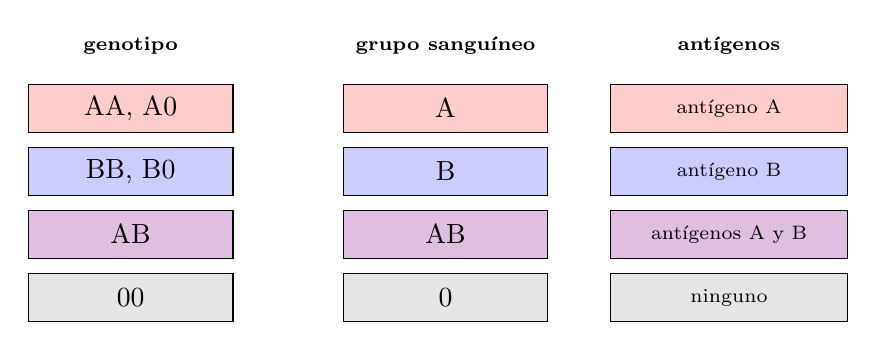
\begin{tikzpicture}

\node[font=\bfseries\scriptsize] at (2.0,3.6) {genotipo}; \node[font=\bfseries\scriptsize] at (6.0,3.6) {grupo sanguíneo}; \node[font=\bfseries\scriptsize] at (9.6,3.6) {antígenos};
\foreach \y/\g/\f/\a/\c in {2.8/{AA, A0}/A/antígeno A/red!20, 2.0/{BB, B0}/B/antígeno B/blue!20, 1.2/AB/AB/antígenos A y B/violet!25, 0.4/00/0/ninguno/gray!20} {\node[draw, fill=\c, minimum width=2.6cm, minimum height=0.6cm] at (2.0,\y) {\g}; \node[draw, fill=\c, minimum width=2.6cm, minimum height=0.6cm] at (6.0,\y) {\f}; \node[draw, fill=\c, minimum width=3.0cm, minimum height=0.6cm, font=\scriptsize] at (9.6,\y) {\a};}

\end{tikzpicture}
\end{document}
